\documentclass[aspectratio=169, xcolor=dvipsnames]{beamer}

% --- Theme Setup ---
\usetheme{Madrid}
\usecolortheme{default}

% --- Packages ---
\usepackage{graphicx}
\usepackage{xcolor}
\usepackage{booktabs}
\usepackage{hyperref}
\usepackage{adjustbox}
\usepackage{amssymb}
\usepackage{longtable}
\usepackage{caption}
\usepackage{tikz}
\usetikzlibrary{mindmap,trees,shadows,arrows.meta,positioning,shapes.geometric,calc}

% --- Title Information ---
\title{Module 01}
\subtitle{Course Overview}
\author{Milav Dabgar}
\institute{www.milav.in}
\date{\today}

\begin{document}

% Title Slide
\begin{frame}
    \titlepage
\end{frame}

\begin{frame}{Module Objectives}
    \begin{itemize}[<+->]
        \item To understand the importance of database management systems in modern day applications
        \item To Know Your Course
    \end{itemize}
\end{frame}

\begin{frame}{Module Outline}
    \begin{itemize}[<+->]
        \item Why Databases?
        \item KYC: Know Your Course
        \item Course Prerequisite
        \item Course Outline
        \item Course Text Book
    \end{itemize}
\end{frame}

\section{Why Databases?}

\begin{frame}
  \vfill
  \centering
  \begin{beamercolorbox}[sep=8pt,center,shadow=true,rounded=true]{title}
    \usebeamerfont{title}Why Databases?\par%
  \end{beamercolorbox}
  \vfill
\end{frame}

\begin{frame}{Database Management System (DBMS)}
    \begin{itemize}[<+->]
        \item DBMS contains information about a particular enterprise
        \item Collection of interrelated data
        \item Set of programs to access the data
        \item An environment that is both convenient and efficient to use
        \item Database Applications:
        \begin{itemize}
            \item Banking: transactions
            \item Airlines: reservations, schedules
            \item Universities: registration, grades
            \item Sales: customers, products, purchases
            \item Online retailers: order tracking, customized recommendations
            \item Manufacturing: production, inventory, orders, supply chain
            \item Human resources: employee records, salaries, tax deductions
        \end{itemize}
        \item Databases can be very large
        \item Databases touch all aspects of our lives
    \end{itemize}
\end{frame}

\begin{frame}{University Database Example}
    \begin{exampleblock}{Application program examples}
        \begin{itemize}[<+->]
            \item Add new students, instructors, and courses
            \item Register students for courses, and generate class rosters
            \item Assign grades to students, compute grade point averages (GPA) and generate transcripts
        \end{itemize}
    \end{exampleblock}
    
    \uncover<4->{
        \vspace{1em}
        \begin{block}{Historical Context}
            In the early days, database applications were built directly on top of file systems
        \end{block}
    }
\end{frame}

\begin{frame}{Drawbacks of using file systems to store data}
    \begin{itemize}[<+->]
        \item Data redundancy and inconsistency
        \begin{itemize}
            \item Multiple file formats, duplication of information in different files
        \end{itemize}
        \item Difficulty in accessing data
        \begin{itemize}
            \item Need to write a new program to carry out each new task
        \end{itemize}
        \item Data isolation
        \begin{itemize}
            \item Multiple files and formats
        \end{itemize}
        \item Integrity problems
        \begin{itemize}
            \item Integrity constraints (e.g., account balance $> 0$) become 'buried' in program code rather than being stated explicitly
            \item Hard to add new constraints or change existing ones
        \end{itemize}
    \end{itemize}
\end{frame}

\begin{frame}{Drawbacks of using file systems to store data (2)}
    \begin{itemize}[<+->]
        \item Atomicity of updates
        \begin{itemize}
            \item Failures may leave database in an inconsistent state with partial updates carried out
            \item Example: Transfer of funds from one account to another should either complete or not happen at all
        \end{itemize}
        \item Concurrent access by multiple users
        \begin{itemize}
            \item Concurrent access needed for performance
            \item Uncontrolled concurrent accesses can lead to inconsistencies
            \item Example: Two people reading a balance (say 100) and updating it by withdrawing money (say 50 each) at the same time
        \end{itemize}
        \item Security problems
        \begin{itemize}
            \item Hard to provide user access to some, but not all, data
        \end{itemize}
    \end{itemize}
    
    \uncover<4->{
        \vspace{0.5em}
        \begin{alertblock}{Solution}
            Database systems offer solutions to all the above problems
        \end{alertblock}
    }
\end{frame}

\section{Know Your Course}

\begin{frame}
  \vfill
  \centering
  \begin{beamercolorbox}[sep=8pt,center,shadow=true,rounded=true]{title}
    \usebeamerfont{title}Know Your Course\par%
  \end{beamercolorbox}
  \vfill
\end{frame}

\begin{frame}{Course Prerequisites: Essential}
    \begin{itemize}[<+->]
        \item \textbf{Set Theory}
        \begin{itemize}
            \item Definition of a Set
            \begin{itemize}
                \item[$\triangleright$] Intensional Definition
                \item[$\triangleright$] Extensional Definition
                \item[$\triangleright$] Set-builder Notation
            \end{itemize}
            \item Membership, Subset, Superset, Power Set, Universal Set
            \item Operations on sets:
            \begin{itemize}
                \item[$\triangleright$] Union, Intersection, Complement, Difference, Cartesian Product
            \end{itemize}
            \item De Morgan's Law
        \end{itemize}
        \item \textbf{Courses}
        \begin{itemize}
            \item[$\triangleright$] MOOCs: Discrete Mathematics: \\
            \url{https://nptel.ac.in/courses/111/106/111106086/}
            \item[$\triangleright$] Online Degree Foundational Course: Mathematics for Data Science I \\
            \url{https://onlinedegree.iitm.ac.in/course_pages/BSCMA1001.html}
        \end{itemize}
    \end{itemize}
\end{frame}

\begin{frame}{Course Prerequisites: Essential (Relations and Functions)}
    \begin{itemize}[<+->]
        \item \textbf{Relations and Functions}
        \begin{itemize}
            \item Definition of Relations
            \item Ordered Pairs and Binary Relations
            \begin{itemize}
                \item[$\triangleright$] Domain and Range
                \item[$\triangleright$] Image, Preimage, Inverse
                \item[$\triangleright$] Properties: Reflexive, Symmetric, Antisymmetric, Transitive, Total
            \end{itemize}
            \item Definition of Functions
            \item Properties of Functions: Injective, Surjective, Bijective
            \item Composition of Functions
            \item Inverse of a Function
        \end{itemize}
        \item \textbf{Courses}
        \begin{itemize}
            \item[$\triangleright$] MOOCs: Discrete Mathematics: \\
            \url{https://nptel.ac.in/courses/111/106/111106086/}
        \end{itemize}
    \end{itemize}
\end{frame}

\begin{frame}{Course Prerequisites: Essential (Propositional Logic)}
    \begin{itemize}[<+->]
        \item \textbf{Propositional Logic}
        \begin{itemize}
            \item Truth Values \& Truth Tables
            \item Operators: conjunction (and), disjunction (or), negation (not), implication, equivalence
            \item Closure under Operations
        \end{itemize}
        \item \textbf{Courses}
        \begin{itemize}
            \item[$\triangleright$] MOOCs: Discrete Mathematics: \\
            \url{https://nptel.ac.in/courses/111/106/111106086/}
        \end{itemize}
    \end{itemize}
\end{frame}

\begin{frame}{Course Prerequisites: Essential (Predicate Logic)}
    \begin{itemize}[<+->]
        \item \textbf{Predicate Logic}
        \begin{itemize}
            \item Predicates
            \item Quantification
            \begin{itemize}
                \item[$\triangleright$] Existential
                \item[$\triangleright$] Universal
            \end{itemize}
        \end{itemize}
        \item \textbf{Courses}
        \begin{itemize}
            \item[$\triangleright$] MOOCs: Discrete Mathematics: \\
            \url{https://nptel.ac.in/courses/111/106/111106086/}
        \end{itemize}
    \end{itemize}
\end{frame}

\begin{frame}{Course Prerequisites: Essential (Data Structures)}
    \begin{itemize}[<+->]
        \item \textbf{Data Structures}
        \begin{itemize}
            \item Array
            \item List
            \item Binary Search Tree
            \begin{itemize}
                \item[$\triangleright$] Balanced Tree
            \end{itemize}
            \item B-Tree
            \item Hash Table / Map
        \end{itemize}
        \item \textbf{Courses}
        \begin{itemize}
            \item[$\triangleright$] MOOCs: Design and Analysis of Algorithms: \\
            \url{https://nptel.ac.in/courses/106/106/106106131/}
            \item[$\triangleright$] MOOCs: Fundamental Algorithms - Design and Analysis: \\
            \url{https://nptel.ac.in/courses/106/105/106105157/}
        \end{itemize}
    \end{itemize}
\end{frame}

\begin{frame}{Course Prerequisites: Essential (Programming)}
    \begin{itemize}[<+->]
        \item \textbf{Programming in Python}
        \item \textbf{Courses}
        \begin{itemize}
            \item[$\triangleright$] Online Degree Foundational Course - Programming in Python \\
            \url{https://onlinedegree.iitm.ac.in/course_pages/BSCCS1002.html}
        \end{itemize}
    \end{itemize}
\end{frame}

\begin{frame}{Course Prerequisites: Desirable}
    \begin{itemize}[<+->]
        \item \textbf{Algorithms and Programming in C}
        \begin{itemize}
            \item Sorting
            \begin{itemize}
                \item[$\triangleright$] Merge Sort
                \item[$\triangleright$] Quick Sort
            \end{itemize}
            \item Search
            \begin{itemize}
                \item[$\triangleright$] Linear Search
                \item[$\triangleright$] Binary Search
                \item[$\triangleright$] Interpolation Search
            \end{itemize}
        \end{itemize}
        \item \textbf{Courses}
        \begin{itemize}
            \item[$\triangleright$] MOOCs: Design and Analysis of Algorithms: \\
            \url{https://nptel.ac.in/courses/106/106/106106131/}
            \item[$\triangleright$] MOOCs: Introduction to Programming in C: \\
            \url{https://nptel.ac.in/courses/106/104/106104128/}
        \end{itemize}
    \end{itemize}
\end{frame}

\begin{frame}{Course Prerequisites: Desirable (OOAD)}
    \begin{itemize}[<+->]
        \item \textbf{Object-Oriented Analysis and Design}
        \item \textbf{Courses}
        \begin{itemize}
            \item[$\triangleright$] MOOCs: Object-Oriented Analysis and Design: \\
            \url{https://nptel.ac.in/courses/106/105/106105153/}
        \end{itemize}
    \end{itemize}
\end{frame}

\begin{frame}{Course Outline}
    \begin{center}
        \resizebox{0.95\textwidth}{!}{
            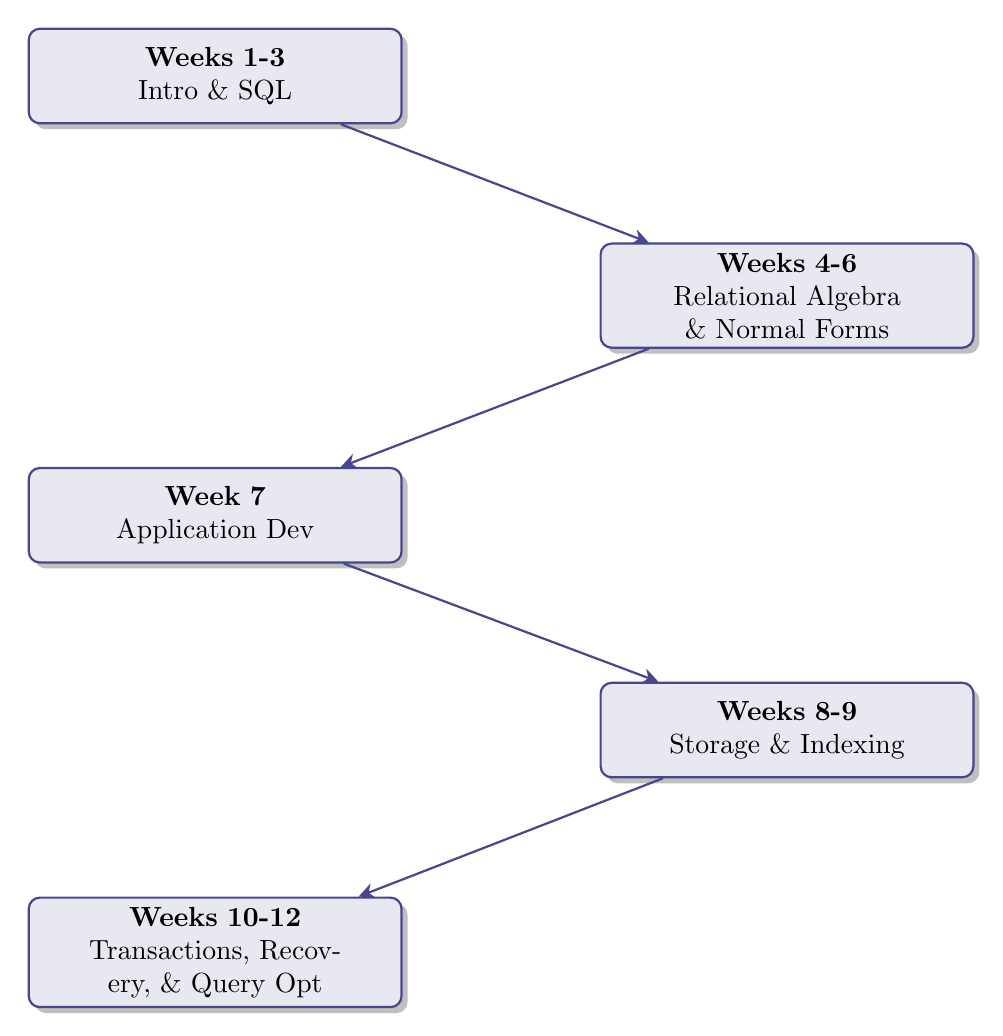
\begin{tikzpicture}[
                node distance=1.5cm and 2.5cm,
                box/.style={rectangle, draw=MidnightBlue!80, fill=MidnightBlue!10, rounded corners, thick, text centered, text width=4.5cm, minimum height=1.2cm, drop shadow},
                arrow/.style={-{Stealth[length=2mm, width=2mm]}, thick, MidnightBlue!80}
            ]
            
            % Nodes
            \node (intro) [box] {\textbf{Weeks 1-3}\\Intro \& SQL};
            \node (model) [box, below right=of intro] {\textbf{Weeks 4-6}\\Relational Algebra \& Normal Forms};
            \node (app) [box, below left=of model] {\textbf{Week 7}\\Application Dev};
            \node (storage) [box, below right=of app] {\textbf{Weeks 8-9}\\Storage \& Indexing};
            \node (trans) [box, below left=of storage] {\textbf{Weeks 10-12}\\Transactions, Recovery, \& Query Opt};
            
            % Arrows
            \draw [arrow] (intro) -- (model);
            \draw [arrow] (model) -- (app);
            \draw [arrow] (app) -- (storage);
            \draw [arrow] (storage) -- (trans);
            
            \end{tikzpicture}
        }
    \end{center}
\end{frame}

\begin{frame}{Course Textbook}
    \begin{columns}
        \begin{column}{0.6\textwidth}
            \textbf{Database System Concepts}\\
            Sixth Edition,\\
            Abraham Silberschatz, Henry Korth, S. Sudarshan,\\
            Publisher: McGraw Hill Education \\
            ISBN: 0073523321\\
            Website: \url{http://db-book.com/}\\
            
            \vspace{1em}
            \textit{7th Edition will also do}
        \end{column}
        \begin{column}{0.4\textwidth}
            \centering
            % Include image here
            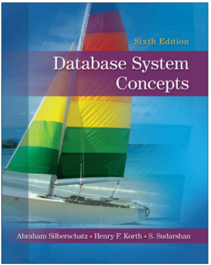
\includegraphics[height=0.7\textheight, keepaspectratio]{../Lecture 1.1 - Course Overview_artifacts/image_000019_ba9c921301f8d9573a8afb3df5ce5eb81c935ef606bbf0c9cc28624218d3ee08.png}
        \end{column}
    \end{columns}
\end{frame}

\begin{frame}{Module Summary}
    \begin{itemize}
        \item Elucidates the importance of database management systems in modern day applications
        \item Introduced various aspects of the Course
    \end{itemize}
    \vspace{2em}
    \begin{center}
    \small \textit{Slides used in this presentation are borrowed from \url{http://db-book.com/} with kind permission of the authors.} \\
    \small \textit{Edited and new slides are marked with 'PPD'.}
    \end{center}
\end{frame}

\end{document}
